\chapter{Boundaries and Fixed objects}
\label{chap:BoundariesAndFixedObjects}

As described before, the base Boundary implementation has been based on the paper "Real-Time Fluid Dynamics for Games" by Jos Stam. This method consists out of the treatment of all boundary cells around the simulation and altering these such that fluids will bounce of these "wall"-cells rather than flow through them.

\begin{figure}[htb!]
    \centering
    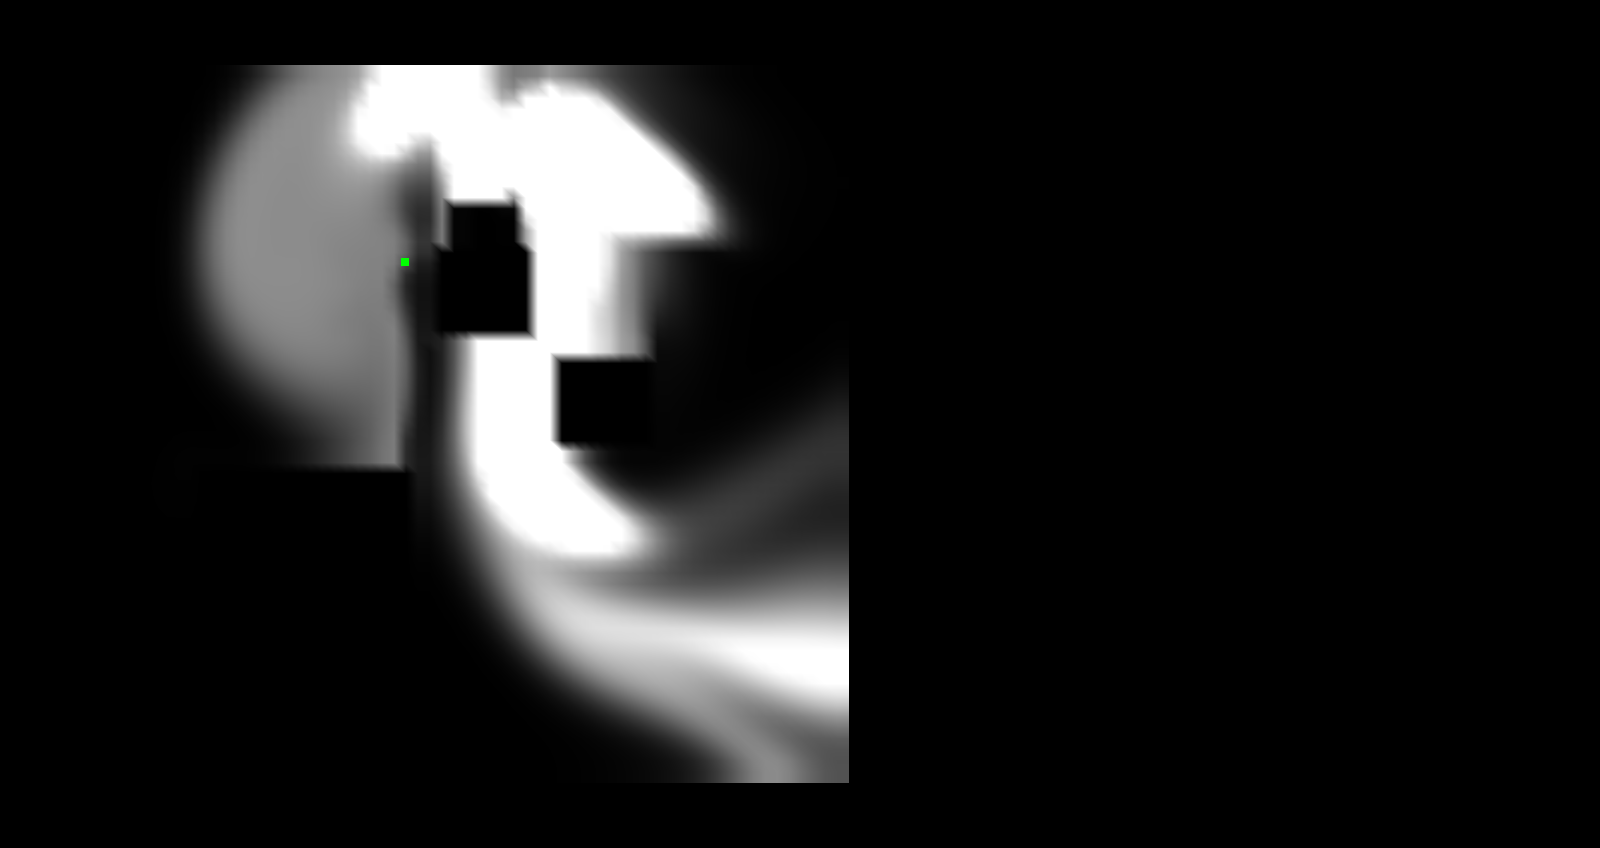
\includegraphics[width=0.6\textwidth]{images/FixedObject}
    \caption{A scene containing solid objects the fluid cannot flow through.}
    \label{fig:Fixed_object}
\end{figure}

To adapt this technique to work for fixed objects within the simulation, a classification is done for every cell. For each cell there are four categories; "Empty", "Invert", "Copy" and "Zero". "Empty" is a classification for a cell that is not part of any sort of object or border. Fluids can flow through this cell normally. "Invert" means an incoming force or density has to be inverted back from where it came originally. This classification needs a source as well in order to know what cell the force has to be directed at. "Copy" copies the velocity or density from a neighbouring cell from a set source. "Zero" cells are cells through which no fluids can flow at all, like the inside of solid objects. The source of the "invert" and "copy" cells is based on the positioning of this cell on the solid object the fluid needs to flow around.

This boundary classification together with their associated source is made and saved in a list for the velocities in horizontal direction and vertical direction as well as the density field. These are done seperately, as different boundary conditions and classifications apply to forces coming from different directions (again as described by Stam).
